\section{Introduction}\label{sec:intro}

Constructing a Euclidean field theory asks for four things at once: a
regularisation of the field, finite-volume laws that remain consistent as the
regularisation is removed, convergence of those laws to a measure on an
infinite-dimensional space, and a verification of the Osterwalder--Schrader
axioms for the limit.  The axioms are a fixed list
\cite{ossier1973,ossier1975}: analyticity, reflection positivity, Euclidean
invariance, clustering and regularity.  Reconstruction then produces a
relativistic quantum field theory from any measure that satisfies them.  The
classical treatments of the programme \cite{gj1987,simon1974,grs1975,nelson1973}
order the four steps differently, but each of them has to pass through all four,
and each of them is careful about which step is proved and which is imported.
Reconstruction is the reason the fourth step matters: the measure is a Euclidean
object, and the quantum field theory is recovered from it, so a theorem that
stops at the measure has proved a Euclidean statement and not yet a quantum
field theory.

The free (Gaussian) layer is the one place where the programme should be
elementary, because the finite-volume law is Gaussian with an explicit
covariance, so the limit question is a question about Gaussian laws rather than
about a general family of measures.  This paper settles the third step there, at
fixed physical volume and in two dimensions.  The torus is flat and periodic,
the covariance is a function of the resolvent, and every quantity that has to
converge is a sum over modes.
The citations above are for position only: no step of the proof is taken from
\cite{ossier1973,ossier1975,minlos1959,gj1987,simon1974,nelson1973,grs1975}.
In particular the classical route to a measure on a space of distributions runs
through the nuclearity of a test space and the Minlos theorem
\cite{minlos1959}; neither is used below, and \cref{sec:carrier} exhibits the
concrete structure that replaces them.

The setting is fixed volume, and that is what gives the problem its shape.  A
lattice with $N$ sites per direction and spacing $a$ samples the torus of
period $L$ exactly when $aN = L$, so the two parameters move together and the
sites crowd into a fixed box rather than filling a growing one.  The index of
the sequence is therefore the number of sites, not the volume, and the limit is
not an infinite-volume limit: the family of laws has one parameter, and the
continuum it approaches is still a fixed-period torus.  What is at issue is
whether the sequence of Borel laws on a completed infinite-dimensional space
converges, and to what.

Two statements are routinely conflated at this point.  The first is convergence
of the finite Fourier marginals: for each finite family of test functions the
law of the resulting finite-dimensional linear image converges.  This is a
statement about finite-dimensional laws, it is what a lattice measurement can
see, and it is a computation in the symbol domain.  The second is convergence of
the laws themselves, as Borel probability measures, on a completed
infinite-dimensional space.  The second does not follow from the first.
Finite-dimensional laws can converge while no limiting Borel probability measure
exists on the completed space, and a family of laws can converge on one
completion and fail to converge on a weaker or stronger one.  The first
statement is therefore evidence for the second and not a substitute for it, and
a proof that establishes only the first has not constructed a measure on the
carrier at all.

Closing that gap needs three things.  One needs a carrier with a Borel structure
and a topology in which the assertions are made; one needs a tightness
argument, since Prokhorov's theorem converts tightness into the existence of
limit points and nothing else does; and one needs a proof that two Borel
probability measures that agree on every cylinder coincide, which is a statement
about the sigma-algebra that the cylinders generate.  This paper supplies all
three concretely, in the symbol and Fourier domain, with no nuclearity theorem
and no Minlos theorem anywhere in the chain.  The carrier is an explicit
weighted sequence space, not a nuclear test space; tightness is a single uniform
moment and a compactness comparison of two weights; cylinder determination is
proved from separability of that space.

The argument has five moves, in this order.

\begin{enumerate}
\item Fix the model and the covariance limit (\cref{sec:lattice},
  \cref{sec:covariance}).  The lattice symbol is computed from the discrete
  Laplacian, the physical-volume Gaussian law is defined, and the covariance
  integrals are proved to converge against a periodic massive resolvent that is
  constructed independently of the Fourier series which is then shown to equal
  it.  The lattice covariance itself is an input object
  (\cref{rem:lattice-input}); what is proved is the limit of its pairings, for
  bounded continuous periodic tests.
\item Build the carrier (\cref{sec:carrier}).  The completion is realised as an
  explicit weighted $\ell^2$ space over the mode lattice, so separability and
  the equality of the cylinder sigma-algebra with the Borel sigma-algebra are
  theorems about a concrete space rather than hypotheses attached to an abstract
  one, and the coordinate maps are continuous and injective
  (\cref{lem:coordinate-embedding}).
\item Prove one moment bound and deduce tightness (\cref{sec:tightness}).  A
  uniform $\HL{2}$ moment with an explicit constant makes the Markov tail
  small, and sublevel sets of the $\HL{2}$ energy are relatively compact in the
  weaker $\HL{3}$ topology, which is exactly what Prokhorov's theorem needs.
\item Identify the finite Fourier marginals (\cref{sec:marginals}).  For each
  finite family of modes the law of the corresponding finite collection of
  coordinates converges to the paired cosine/sine Gaussian law whose covariance
  is the resolvent pairing of step~1.
\item Identify the limit and pass to the whole sequence
  (\cref{sec:identification}, \cref{sec:main}).  Every subsequential limit
  inherits those marginals by continuity of the cylinder maps; cylinder
  uniqueness gives one limit for all of them; and the subsequence criterion
  upgrades subsequential convergence to convergence of the sequence.
\end{enumerate}

\begin{figure}[t]
\centering
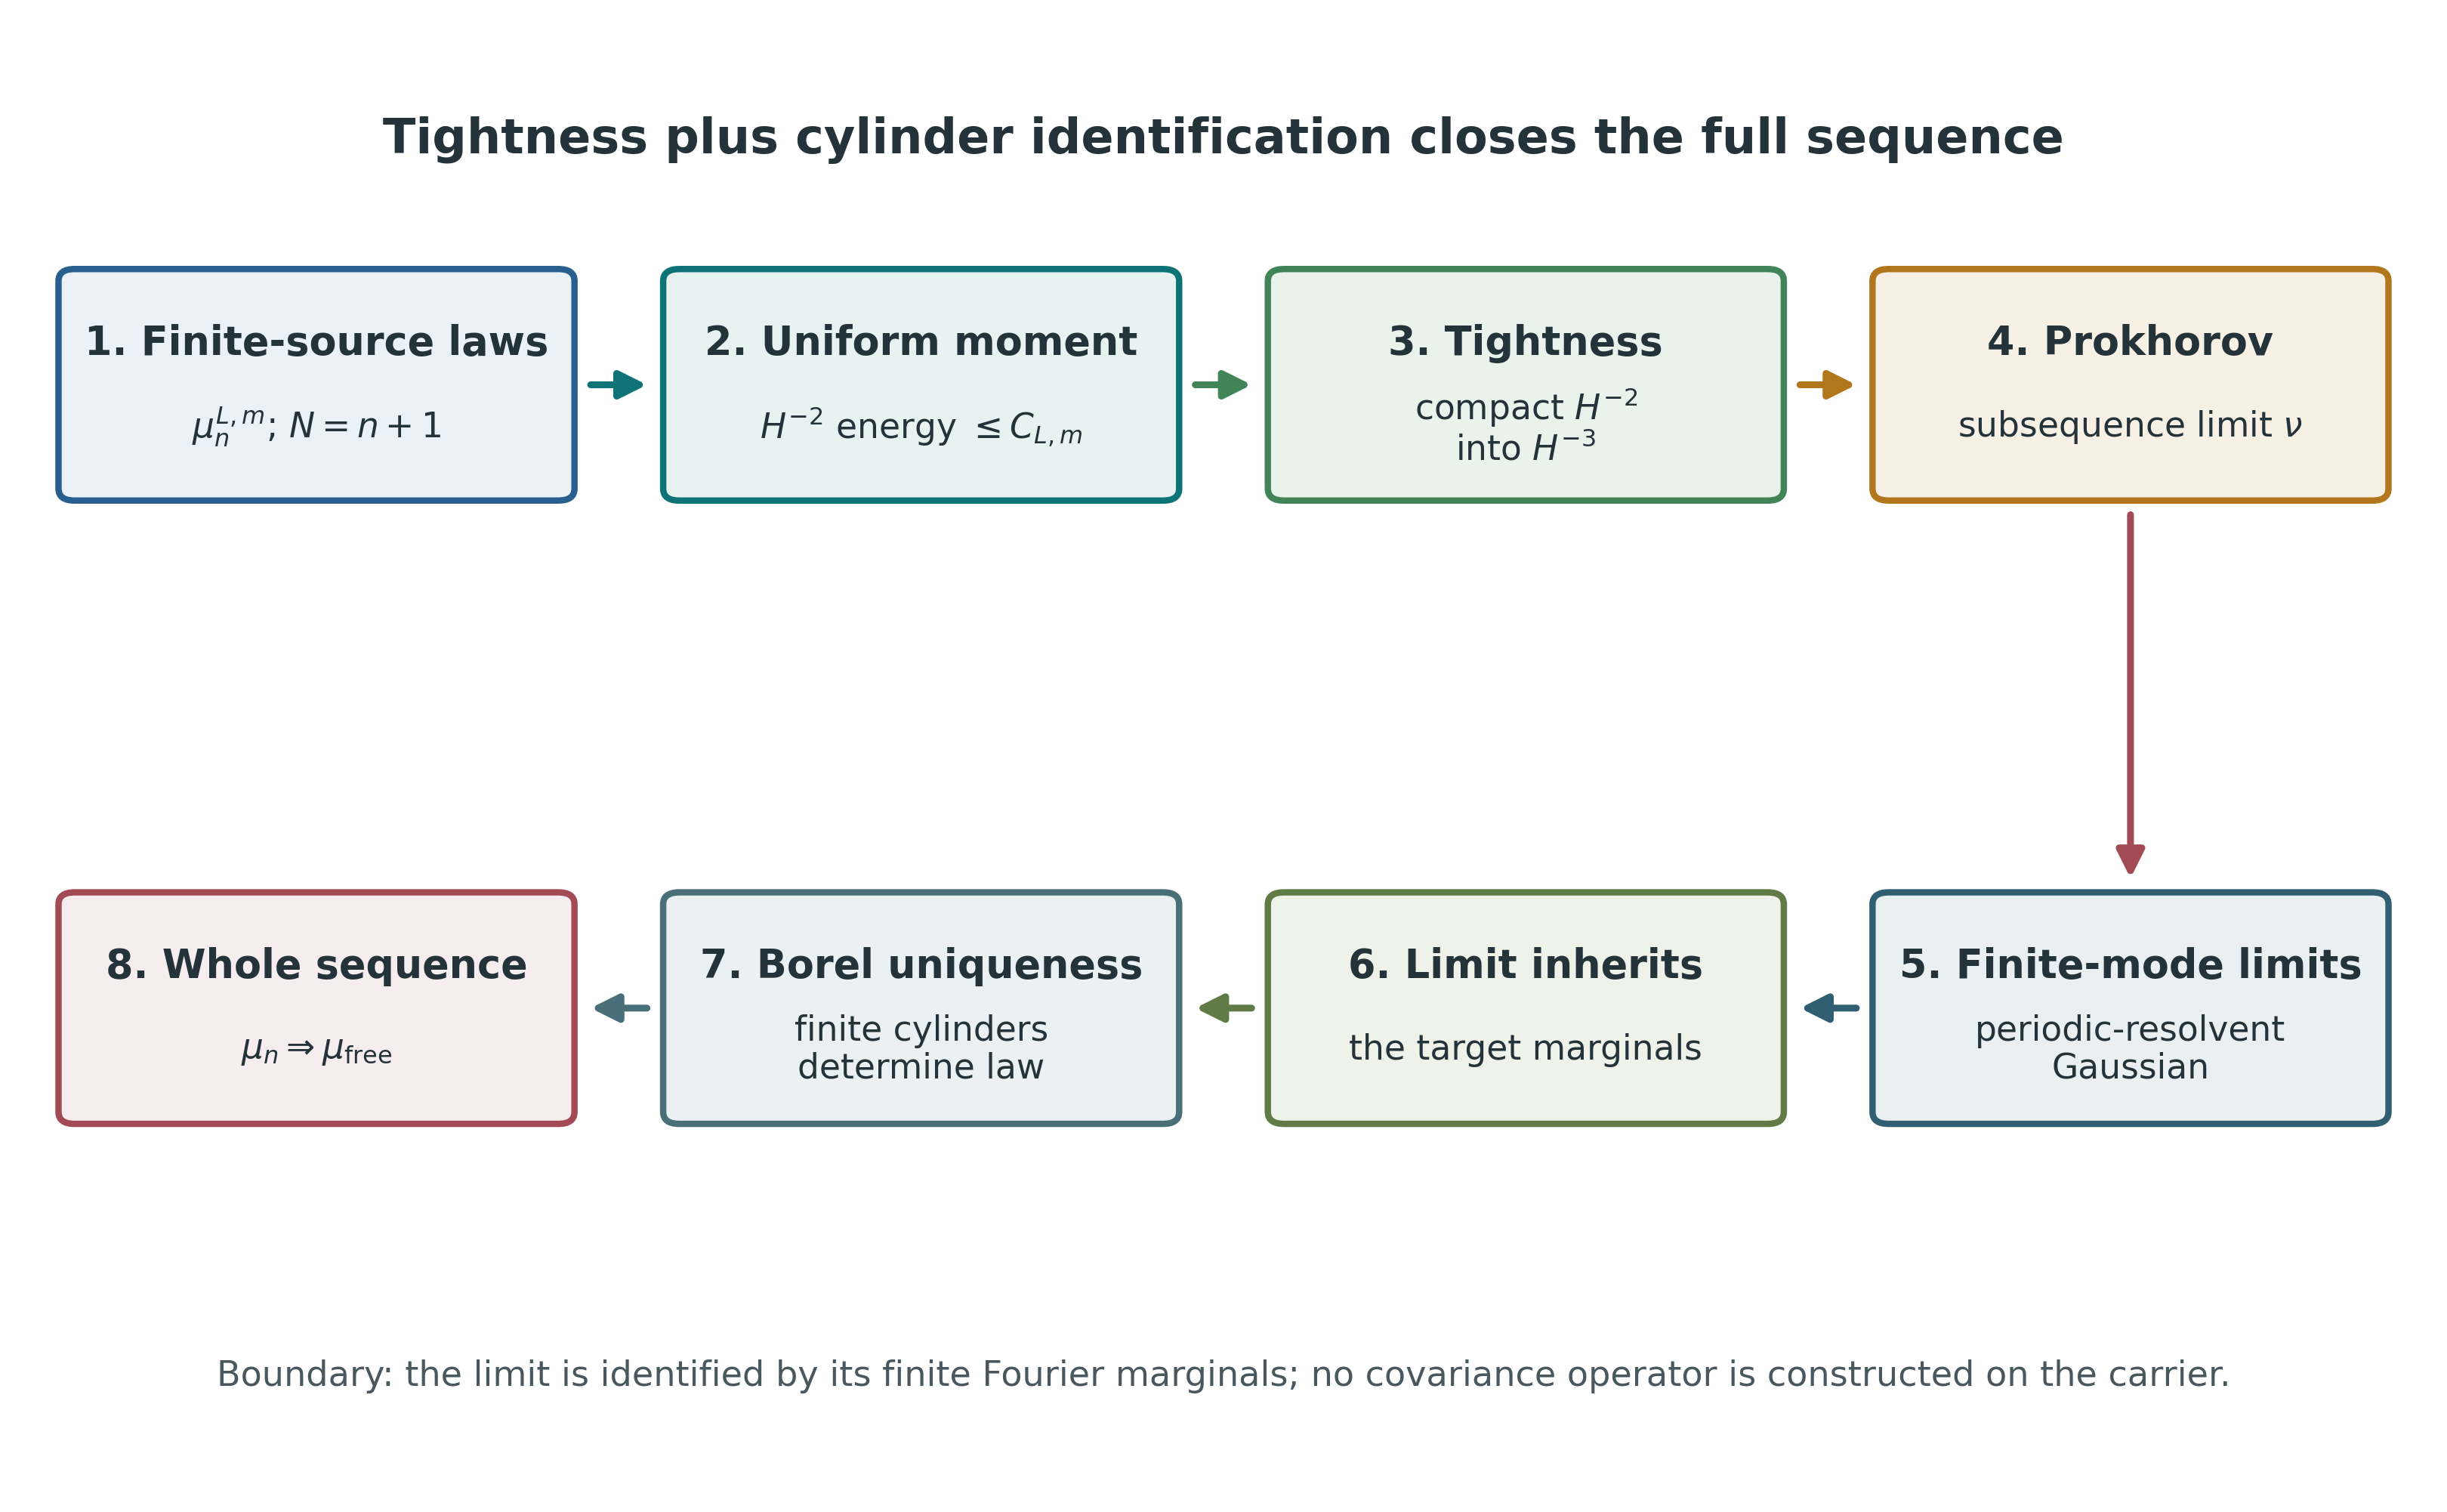
\includegraphics[width=\linewidth]{figures/weak_limit_spine.png}
\caption{The spine of the limit argument. The first box is the point of departure, the finite-source lattice laws; the seven after it carry the argument: the uniform $H^{-2}$ moment; tightness on the carrier; Prokhorov extraction of a subsequential limit; the finite-mode limits from the marginal computations; the limit inherits the target marginals; cylinder-to-Borel uniqueness identifies that limit; and whole-sequence convergence closes it. The last step is the whole-sequence conclusion, not merely a subsequential one. Two inputs are not drawn, because they are settled before this half begins: the carrier construction (move~2 of \cref{sec:intro}) and the covariance limit (part of move~1), which is where the target covariance comes from. Two reading notes. The figure's own footer annotation calls the total-carrier lift a separate input that is not used here; that annotation records the development's implementation choice and is superseded by \cref{lem:lift-representative} and \cref{rem:lift-development}, which prove the paper's lift total and Borel outright. And the figure labels the mass $M$ where the text writes $m$; the index $n$ is the text's own mesh index, not the text's $N$.}
\label{fig:spine}
\end{figure}


The figure shows the spine of the argument, from the lattice laws through the
moment bound and tightness to the whole-sequence conclusion, in the order in
which the steps are proved.

What makes the argument checkable rather than merely correct is the following.

\begin{itemize}
\item The covariance limit (\cref{thm:covariance-limit}) is proved against the
  resolvent of \cref{lem:resolvent}, which is built from an energy identity and
  a Riesz adjoint and is therefore available before any Fourier series is
  written.  The symbol is an output of that construction, not a postulate that
  the lattice limit is then matched to.  The limit of the sampled covariance is
  therefore settled independently of what the series says it is.
\item The carrier is the explicit weighted $\ell^2$ space of
  \cref{def:carrier-hminus3}.  Separability (\cref{thm:separable}) and the
  equality of cylinder and Borel sigma-algebras (\cref{thm:cylinder-borel}) are
  proved for that space, so the two structural facts that a measure-theoretic
  limit normally assumes are theorems here.
\item The conclusion (\cref{thm:main}) is about the whole sequence, and
  \cref{cor:uniqueness} shows that no subsequence can produce a different limit.
  The two quantitative inputs are the uniform moment (\cref{thm:uniform-moment})
  and the marginal limits (\cref{thm:finite-family}); the identification step
  rests on \cref{thm:cylinder-uniqueness}.
\item The target law of each finite family is computed and not selected.  Its
  characteristic function is derived from the resolvent pairing of step~1
  (\cref{thm:char-function}) and its covariance entries are matched to that
  pairing, so the marginal limits are a consequence of the covariance limit
  rather than a second, independent assumption about what the limit should be.
\end{itemize}

Two items are stated in the underlying documents without a paper-level
derivation, and are derived in full here: the uniform trace constant behind the
moment bound (\cref{lem:trace-constant}) and the entrywise identification of the
paired cosine/sine covariance matrix (\cref{lem:hC-identification}).  Both are
elementary once the normalisation of the lattice covariance is fixed, and both
are needed before the tightness and marginal steps can be completed.

The scope of the result is deliberately narrow.  What converges is the
finite-source Fourier pushforward $\mu_N$ of the lattice Gaussian law, which
\cref{lem:lift-representative} identifies as the law of a Borel carrier-valued
map of the lattice field, so ``the lattice field laws converge'' is asserted in
exactly that sense and no other: the statement is about the law of the Fourier
coefficient sequence, not about a particular total lift of the development
(\cref{rem:lift-development}).  No rate of convergence,
no exponential tail and no quantitative modulus is claimed: the tightness
argument is Markov's inequality applied to a second moment of the norm, and nothing else.  No
interacting ultraviolet limit and no Osterwalder--Schrader reconstruction is
proved; the theory constructed here is the free one.  The carrier, its weights
and every object in the measure limit are two-dimensional, and no dimensional
generalisation of them is claimed.  \Cref{sec:scope} states the boundary in full
and \cref{sec:lean-boundary} states which layer of the argument is
machine-checked.
